\documentclass{article}

\usepackage{amsmath}
\usepackage{graphicx}
\usepackage{bbold}


\title{Examination project 14: Inverse iteration method\\ \small Practical Programming and Numerical Methods 2020}
\author{Marco Majland}
\begin{document}
	\maketitle
	\noindent
	The objective of the project is to iteratively calculate the eigenvalue of a given real symmetric matrix, $\mathbf{A}$, closest to an input eigenvalue and its associated eigenvector. This is done using the inverse iteration method which is an improvement of the power iteration method. By shifting the matrix equation of the power method, one obtains the inverse iteration method.\\
	Let $\mathbf{A}$ denote a real  symmetric matrix of dimension $n\times n$ and the initial guess of the eigenvalue and eigenvector be $s$ and $\mathbf{u}$ (normalized), respectively. The inverse iteration method is then given by
	\begin{equation}
		(\mathbf{A} - s\mathbb{1})\mathbf{v} = \mathbf{u}
		\label{eq:inverse_iteration}
	\end{equation}
	where $\mathbf{v}$ is the refined eigenvector of $\mathbf{A}$. In the implementation of the inverse iteration algorithm, the above linear matrix equation is solved using QR decomposition. During the iterations, one may update the matrix in Eq. \ref{eq:inverse_iteration} used in solving for the iterated vector, $\mathbf{v}$. The update, however, requires further QR decomposition at the cost of $O(n^3)$ operations, although this may yield faster convergence.\\
	In the following, the implementation is tested in two different ways. First, the method is investigated to work as intended for initial eigenvalues/eigenvectors deviating slightly from the target eigenvalue/eigenvector. Here, it is verified that the iterated eigenvalue actually converges to eigenvalues of $\mathbf{A}$. A description of the procedure is described in the following section. Numerical results are presented in \texttt{test\_out.txt}.
	\subsection*{Test of the algorithm}
	To perform a test of the algorithm, a random real symmetric matrix $\mathbf{A}$ of dimensions $30\times 30$ is generated. For comparison, $\mathbf{A}$ is diagonalized using the Jacobi diagonalization procedure implemented in problems 4 (\texttt{/root/numerical/4-eigen}). A random eigenvalue, $e_{i}$, is chosen from the sequence of eigenvalues produced in the Jacobi procedure. The initial guess of the sought eigenvalue is parametrized as $s_{0} = \delta e_{i}$ where $\delta$ is the deviation. Apparently, the inverse iteration method is sensitive to the deviation from the sought eigenvalue which is demonstrated later in the project. In this test of the algorithm, no Rayleigh updates are made for simplicity. Thus, Eq. \ref{eq:inverse_iteration} is solved iteratively until convergence. Since the resulting scalar $s$ and vector $\mathbf{v}$ should be an eigenvalue and eigenvector of $\mathbf{A}$, respectively, the convergence criteria for the absolute and relative accuracies are
	\begin{equation}
		\textrm{norm}\Big(\mathbf{A}\mathbf{v_{i}} - s\mathbf{v_{i}}\Big)\leq\tau\quad\textrm{(absolute)}
	\end{equation}
	and
	\begin{equation}
	\frac{\textrm{norm}\Big(\mathbf{A}\mathbf{v_{i}} - s\mathbf{v_{i}}\Big)}{\textrm{norm}(\mathbf{A}\mathbf{v_{i}}) + \textrm{norm}(s\mathbf{v_{i}})}\leq\frac{\epsilon}{2}\quad\textrm{(relative)}.
	\label{eq:relative_error}
	\end{equation}
	Such an example is presented in the output file \texttt{/root/numerical/exam/test\_out.txt}. The file contains the following information. The random matrix $\mathbf{A}$ is generated and a random eigenvalue index is chosen after the Jacobi diagonalization. To track convergence to the correct eigenvalue, the eigenvalues closest to $e_{i}$ in question are presented. The deviation $\delta$ is chosen, in the example, $\delta = 1.05$ which implies the initial eigenvalue guess deviates $5\%$ from the Jacobi eigenvalue which is assumed to be the correct eigenvalue. Absolute and relative accuracies are chosen to be $\tau=\epsilon=10^{-6}$. Two different approaches are made to the initial guess of the eigenvector. First, a random normalized vector is chosen. Second, the corresponding eigenvector of the Jacobi diagonalization for the sought eigenvalue is chosen, but the entries are deviated with $\delta$. Then, the iteration result is presented. To ensure the correct eigenvector has been found, the scalar quantity
	\begin{equation}
		s = \mathbf{v^{T}Av}
	\end{equation}
	is calculated and must equal the iterated eigenvalue since $\mathbf{v}$ is an eigenvector of $\mathbf{A}$ if the iteration procedure is succesful.\\
	To investigate whether the eigenvalue may have converged to a neighbouring eigenvalue in the spectrum of $\mathbf{A}$, the deviation from these eigenvalues is also calculated.\\
	In other words, let the target eigenvalue be $e_{i}$ and neighbouring eigenvalues $e_{i-1},e_{i+1}$. The errors are then
	\begin{align}
		\mathrm{error}_{i-1} &= |e_{i-1} - s| \\
		\mathrm{error}_{i} &= |e_{i} - s| \\		
		\mathrm{error}_{i+1} &= |e_{i+1} - s|
	\end{align}
	Thus, if one of the errors are much smaller than the other errors, one may conclude convergence of the iteration method to the corresponding eigenvalue.\\
	$\mathbf{NOTE:}$ Only random eigenvalues up to dimension-1 are picked since the file compares the calculated eigenvalue to the neighbouring eigenvalues. Thus, if the program picks the last eigenvalue in the spectrum, this will return an error.
	\subsection*{Test of convergence}
	The inverse iteration method converges slower and potentially to a wrong eigenvalue if the initial deviation is too large. Thus, by picking an eigenvalue closer to the sought eigenvalue, one achieves faster convergence. Furthermore, using the Rayleigh update, one may achieve even faster convergence. To demonstrate this, the inverse iteration method was applied on a random real symmetric matrix $\mathbf{A}$ for different initial deviations, with and without the Rayleigh update. For these calculations, the deviations were $\delta=1.01,1.02,1.03$. The convergence of the relative error, given by Eq. \ref{eq:relative_error}, is depicted in Fig. \ref{fig:convergence}. This quantity, however, only describes convergence to a given eigenvalue/eigenvector, not necessarily to the target eigenvalue/eigenvector. Thus, to check whether the algorithm actually converges to the target eigenvalue and not some neigbouring eigenvalue, convergence to the initial Jacobi eigenvalue is tested. The results are depicted in Fig. \ref{fig:convergence2}. As can be seen, if the quantity converges to a small number, the corresponding calculation converges to the target eigenvalue. If not, the algorithm may have converged to a neighbouring eigenvalue.\\
	To investigate the same convergences for higher deviations, calculations with $\delta=1.05,1.075,1.10$ were made and are depicted analogously to the above in Figs. \ref{fig:convergence3} and \ref{fig:convergence4}.\\
	For all the above calculations, the matrix dimension is 30, $\tau=\epsilon=10^{-6}$. For the calculations in which the Rayleigh update is performed, it is performed for every iteration.
	\begin{figure}
		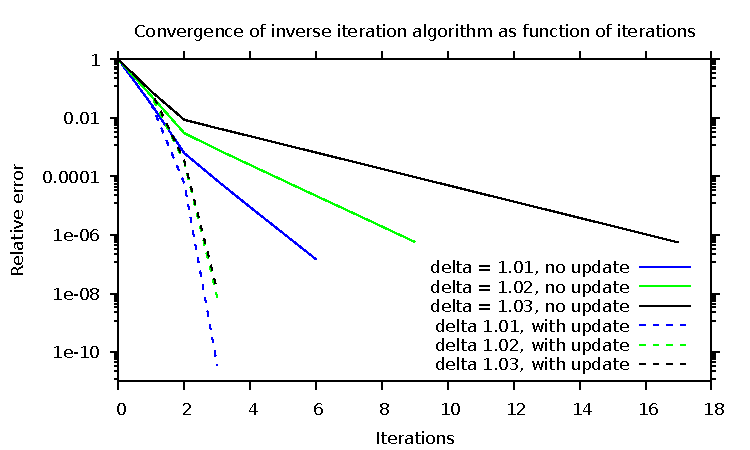
\includegraphics[]{../Convergence.pdf}
		\caption{Relative error as function of iterations for the inverse iteration method applied on a random real symmetric matrix $\mathbf{A}$ with and without the Rayleigh update. This convergence implies convergence to a given eigenvalue/eigenvector.}
		\label{fig:convergence}
	\end{figure}
	\begin{figure}
		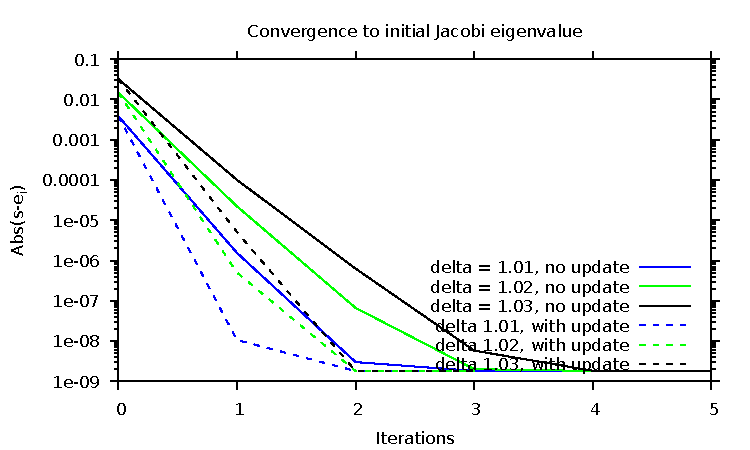
\includegraphics[]{../Convergence2.pdf}
		\caption{Deviation of iterating eigenvalue relative to the initial Jacobi eigenvalue. This convergence demonstrates the convergence to the target eigenvalue.}
		\label{fig:convergence2}
	\end{figure}
	\begin{figure}
		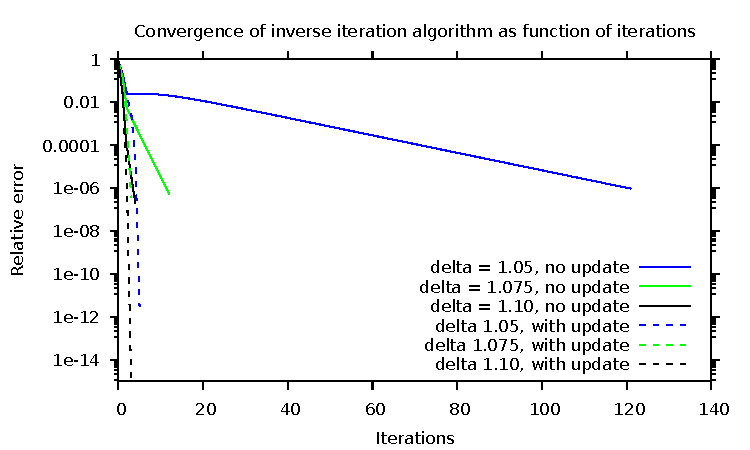
\includegraphics[]{../Convergence3.pdf}
		\caption{Relative error as function of iterations for the inverse iteration method applied on a random real symmetric matrix $\mathbf{A}$ with and without the Rayleigh update. This convergence implies convergence to a given eigenvalue/eigenvector.}
		\label{fig:convergence3}
	\end{figure}
	\begin{figure}
		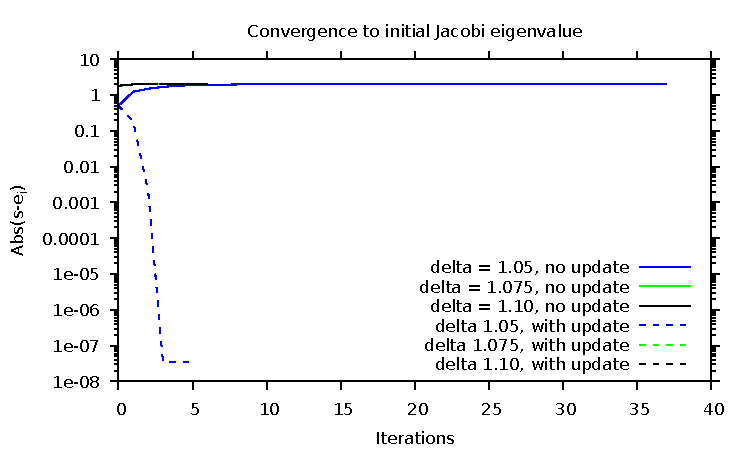
\includegraphics[]{../Convergence4.pdf}
		\caption{Deviation of iterating eigenvalue relative to the initial Jacobi eigenvalue. This convergence demonstrates the convergence to the target eigenvalue.}
		\label{fig:convergence4}
	\end{figure}
\end{document}
